%----------------------------------------------------------------------------------------
%	PACKAGES AND THEMES
%----------------------------------------------------------------------------------------
\documentclass[14pt]{beamer}
\setbeamertemplate{bibliography item}[text]
\mode<presentation> 
{
    \usetheme{Madrid}
    %\usefonttheme{structuresmallcapsserif} 
    %\usetheme{Berlin}
    %\usecolortheme{beaver}
}
\usepackage{graphicx,ctex} % Allows including images
\usepackage{xcolor}
\usepackage{listings}
\lstset{
    basicstyle=\ttfamily\scriptsize,  % 使用脚注大小的等宽字体
    showstringspaces=false,              % 不显示字符串中的空格
    commentstyle=\color{green},          % 注释的颜色为绿色
    keywordstyle=\color{purple},         % 关键字的颜色为紫色
    numbers=left,                        % 在左侧显示行号
    numberstyle=\tiny\color{gray}       % 行号的样式
}
\logo{
\includegraphics[height=0.5cm]{./figure/whulogo.eps}}

%----------------------------------------------------------------------------------------
%	TITLE PAGE
%----------------------------------------------------------------------------------------
\title[PintOS] %optional
{Project 0: Getting Real}

\author % (optional, for multiple authors)
{陈震雄}

\institute % (optional)
{
 武汉大学 
}

\date % (optional)
{\today}

%----------------------------------------------------------------------------------------
%	Highlight the title of the current section
%----------------------------------------------------------------------------------------
\AtBeginSection[]
{
    \begin{frame}
        \frametitle{Table of Contents}
        \tableofcontents[currentsection]
    \end{frame}
}

\begin{document}

% insert title page---------------------------
\frame{\titlepage}

%insert contents------------------------------
\begin{frame}
    \frametitle{Table of Contents}
    \tableofcontents
\end{frame}

\section{Task 1: Booting Pintos}

% insert a sample frame without animation--------------------------------
\begin{frame}
    \frametitle{Exercise 1.1}
    \begin{itemize}
        \item Take screenshots of the successful booting of Pintos in QEMU and Bochs.
    \end{itemize}
    \begin{figure}
        \centering
        \begin{minipage}{0.8\textwidth}
            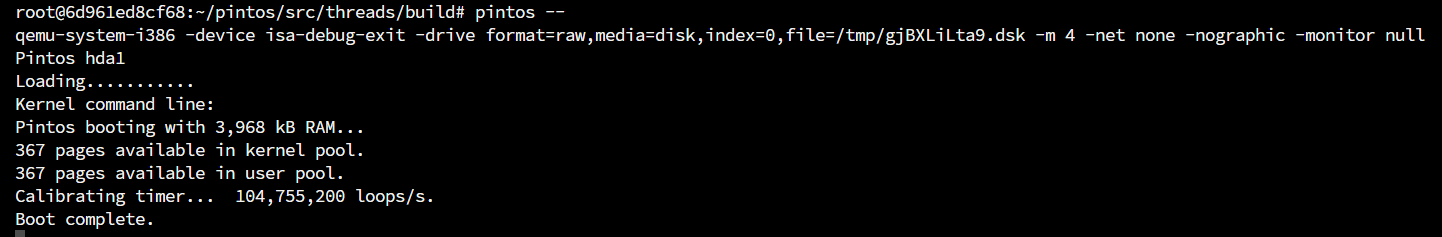
\includegraphics[width=\linewidth]{figure/boot1.png}
        \end{minipage}
        \vspace{1cm} % 添加垂直间距
        \begin{minipage}{0.8\textwidth}
            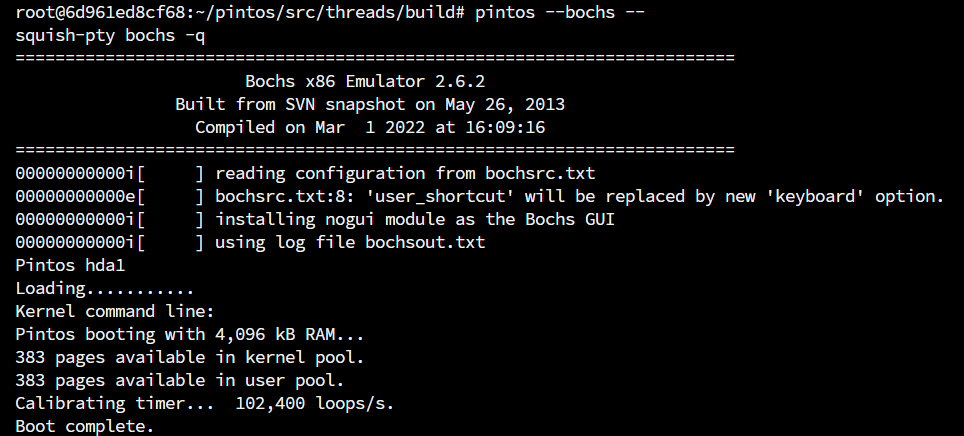
\includegraphics[width=\linewidth]{figure/boot2.png}
        \end{minipage}
    \end{figure}
\end{frame}
%----------------------------------------
\section{Task 2: Debugging}
\begin{frame}[fragile]
    \frametitle{Exercise 2.1}
    \begin{itemize}
        \item What is the first instruction that gets executed?
    \end{itemize}
    \begin{block}{}
        \begin{lstlisting}[language=bash]
(gdb) debugpintos
The target architecture is assumed to be i8086
[f000:fff0]    0xffff0: ljmp   $0x3630,$0xf000e05b
0x0000fff0 in ?? ()
        \end{lstlisting}
    \end{block}
\end{frame}
%--------------------------------------------------
\begin{frame}{Exercise 2.1}
\begin{figure}
    \centering
    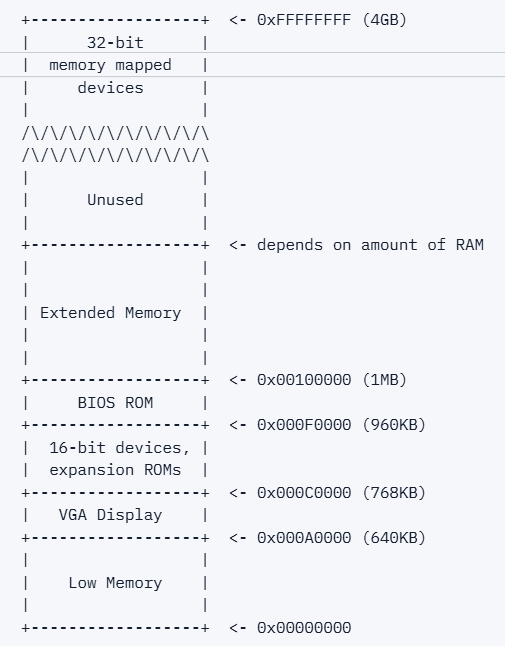
\includegraphics[width=0.5\linewidth]{figure/memlayout.png}
    \caption{memlayout}
\end{figure}
\end{frame}
%--------------------------------------------------
\begin{frame}[fragile]{Exercise 2.2}
\begin{itemize}
    \item How does the bootloader read disk sectors? In particular, what BIOS interrupt is used?
\end{itemize}
    \begin{block}{}
        \begin{lstlisting}[language=bash]
(gdb) break *0x7c00 
Breakpoint 1 at 0x7c00
(gdb) c
Continuing.
[   0:7c00] => 0x7c00:  sub    %eax,%eax
Breakpoint 1, 0x00007c00 in ?? ()
(gdb) x/8i $pc
=> 0x7c00:      sub    %eax,%eax
   0x7c02:      mov    %eax,%ds
   0x7c04:      mov    %eax,%ss
   0x7c06:      mov    $0xf000,%sp
   0x7c0a:      add    %al,(%eax)
   0x7c0c:      sub    %edx,%edx
   0x7c0e:      mov    $0xe3,%al
   0x7c10:      int    $0x14
   ...
   call read_sector
        \end{lstlisting}
    \end{block}
\end{frame}
%-----------------------------------------------
\begin{frame}[fragile]{Exercise 2.2}
    \begin{block}{loader.S}
        \begin{lstlisting}[language={[x86masm]Assembler}]
read_sector:
    pusha
    sub %ax, %ax
    push %ax            # LBA sector number [48:63]
    push %ax            # LBA sector number [32:47]
    push %ebx           # LBA sector number [0:31]
    push %es            # Buffer segment
    push %ax            # Buffer offset (always 0)
    push $1             # Number of sectors to read
    push $16            # Packet size
    mov $0x42, %ah     # Extended read
    mov %sp, %si       # DS:SI -> packet
    int $0x13          # Error code in CF
    popa                # Pop 16 bytes, preserve flags
        \end{lstlisting}
    \end{block}
\end{frame}
\begin{frame}[fragile]{Exercise 2.2}
Reading hard disk sectors requires the use of the functions provided by BIOS. Specifically, as mentioned in the title, it triggers a BIOS interrupt. The instruction is located in line 242 (red box in the figure). A complete interrupt table is available for query under the BIOS interrupt call entry on Wikipedia:
    \begin{figure}
        \centering
        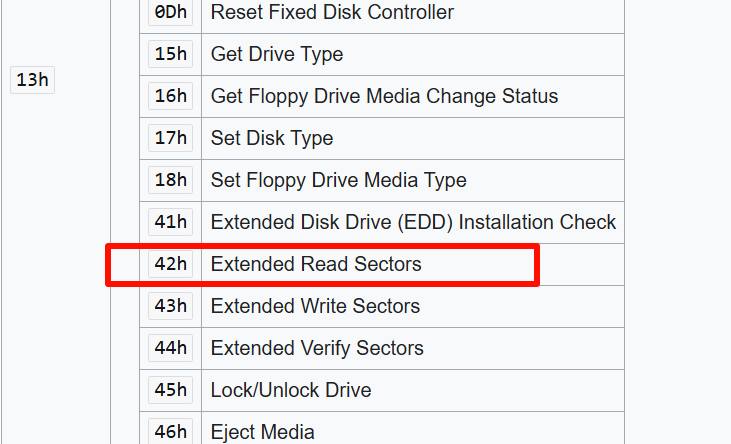
\includegraphics[width=0.5\linewidth]{figure/13h.png}
        \end{figure}

\end{frame}
%-----------------------------------------------
\begin{frame}[fragile]{Exercise 2.2}
\begin{itemize}
    \item How does the bootloader decide whether it successfully finds the Pintos kernel?
\end{itemize}
\end{frame}
%-----------------------------------------------
\begin{frame}[fragile]{Exercise 2.2}
    \begin{block}{}
        \begin{lstlisting}[language={[x86masm]Assembler}]
    # Check for MBR signature--if not present, it's not a
    # partitioned hard disk.
    cmpw $0xaa55, %es:510
    jne next_drive

    mov $446, %si   # Offset of partition table entry 1.
    mov $'1', %al
check_partition:
    # Is it an unused partition?
    cmpl $0, %es:(%si)
    je next_partition
    # Print [1-4].
    call putc

    # Is it a Pintos kernel partition?
    cmpb $0x20, %es:4(%si)
    jne next_partition

    # Is it a bootable partition?
    cmpb $0x80, %es:(%si)
    je load_kernel
        \end{lstlisting}
    \end{block}
\end{frame}
%-----------------------------------------------
\begin{frame}[fragile]{Exercise 2.2}
    \begin{block}{}
        \begin{lstlisting}[language={[x86masm]Assembler}]
next_partition:
 # No match for this partition, go on to the next one.
    add $16, %si   # Offset to next partition table entry.
    inc %al
    cmp $510, %si
    jb check_partition
 next_drive:
 # No match on this drive, go on to the next one.
    inc %dl
    jnc read_mbr
        \end{lstlisting}
    \end{block}
    \begin{figure}
        \centering
        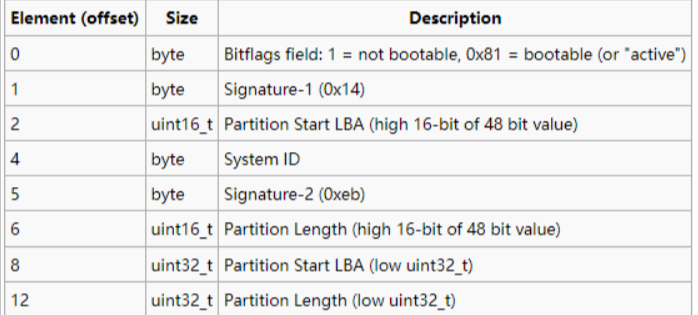
\includegraphics[width=0.6\linewidth]{figure/partition.png}
    \end{figure}
\end{frame}
%-----------------------------------------------
\begin{frame}[fragile]{Exercise 2.2}
\begin{itemize}
    \item What happens when the bootloader could not find the Pintos kernel?
\end{itemize}
\begin{block}{}
    \begin{lstlisting}[language={[x86masm]Assembler}]
no_such_drive:
no_boot_partition:
 # Didn't find a Pintos kernel partition anywhere, give up.
 call puts
 .string "\rNot found\r"

 # Notify BIOS that boot failed.  See [IntrList].
 int $0x18
        \end{lstlisting}
    \end{block}
\end{frame}
%-----------------------------------------------
\begin{frame}[fragile]{Exercise 2.2}
    \begin{figure}
        \centering
        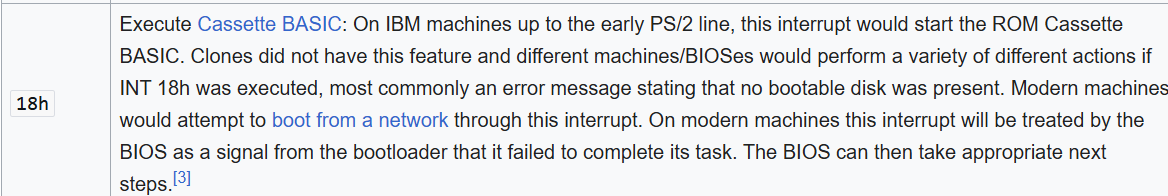
\includegraphics[width=\linewidth]{figure/NotFound.png}

    \end{figure}
\end{frame}
%-----------------------------------------------
\begin{frame}[fragile]{Exercise 2.2}
\begin{itemize}
    \item At what point and how exactly does the bootloader transfer control to the Pintos kernel?
\end{itemize}

\end{frame}
%-----------------------------------------------
\begin{frame}[fragile]{Exercise 2.2}
    \begin{block}{loader.S}
        \begin{lstlisting}[language={[x86masm]Assembler}]
load_kernel:
    ...
    mov $0x2000, %ax
    mov %ax, %es
    mov %es:0x18, %dx
    mov %dx, start
    movw $0x2000, start + 2
    ljmp *start
        \end{lstlisting}
    \end{block}
\begin{figure}
    \centering
    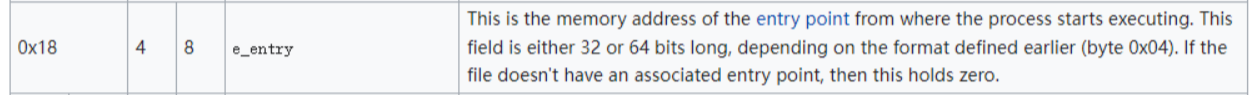
\includegraphics[width=\linewidth]{figure/ELF0x18.png}

\end{figure}
\end{frame}
%-----------------------------------------------
\begin{frame}[fragile]{Exercise 2.3}
\begin{itemize}
    \item At the entry of pintos\_init(), what is** **the value of the expression init\_page\_dir[pd\_no(ptov(0))] in hexadecimal format?
\end{itemize}
\end{frame}
%-----------------------------------------------
\begin{frame}[fragile]{Exercise 2.3}
\begin{block}{}
    \begin{lstlisting}
(gdb) b pintos_init
Breakpoint 1 at 0xc00202b6: file ../../threads/init.c, line 78.
(gdb) continue
Continuing.
The target architecture is assumed to be i386
=> 0xc00202b6 <pintos_init>:    push   %ebp

Breakpoint 1, pintos_init () at ../../threads/init.c:78
(gdb) p init_page_dir[pd_no(ptov(0))]
=> 0xc000efef:  int3   
=> 0xc000efef:  int3   
$1 = 0
    \end{lstlisting}
\end{block}
\end{frame}
%-----------------------------------------------
\begin{frame}[fragile]{Exercise 2.3}
\begin{itemize}
    \item When palloc\_get\_page() is called for the first time,
\begin{itemize}
    \item what does the call stack look like?

\item what is the return value in hexadecimal format?

\item  what is the value of expression init\_page\_dir[pd\_no(ptov(0))] in hexadecimal format?
\end{itemize}

\end{itemize}
\end{frame}
%-----------------------------------------------
\begin{frame}[fragile]{Exercise 2.3}
    \begin{lstlisting}
(gdb) b palloc_get_page
Breakpoint 2 at 0xc002311a: file ../../threads/palloc.c, line 113.
(gdb) continue
Continuing.
=> 0xc002311a <palloc_get_page+6>:      sub    $0x8,%esp
Breakpoint 2, palloc_get_page (flags=(PAL_ASSERT | PAL_ZERO))
at ../../threads/palloc.c:113
(gdb) bt
#0  palloc_get_page (flags=(PAL_ASSERT | PAL_ZERO)) at 
../../threads/palloc.c:113
#1  0xc00203aa in paging_init () at ../../threads/init.c:168
#2  0xc002031b in pintos_init () at ../../threads/init.c:100
#3  0xc002013d in start () at ../../threads/start.S:180
(gdb) fin
Run till exit from #0  palloc_get_page (flags=(PAL_ASSERT | PAL_ZERO)) at 
../../threads/palloc.c:113
=> 0xc00203aa <paging_init+17>: add    $0x10,%esp
0xc00203aa in paging_init () at ../../threads/init.c:168
Value returned is $2 = (void *) 0xc0101000
(gdb) p/x init_page_dir[pd_no(ptov(0))]
=> 0xc000ef8f:  int3   
=> 0xc000ef8f:  int3   
$3 = 0x0
    \end{lstlisting}
\end{frame}
%-----------------------------------------------
\begin{frame}[fragile]{Exercise 2.3}
\begin{itemize}
    \item When palloc\_get\_page() is called for the third time,
\begin{itemize}
    \item what does the call stack look like?

\item what is the return value in hexadecimal format?

\item what is the value of expression init\_page\_dir[pd\_no(ptov(0))] in hexadecimal format?
\end{itemize}

\end{itemize}

\end{frame}
%-----------------------------------------------
\begin{frame}[fragile]{Exercise 2.3}
\begin{block}{}
\begin{lstlisting}
(gdb) bt
#0  palloc_get_page (flags=PAL_ZERO) at ../../threads/palloc.c:113
#1  0xc0020a81 in thread_create (name=0xc002e895 "idle", priority=0, 
function=0xc0020eb0 <idle>, aux=0xc000efbc) at ../../threads
/thread.c:178
#2  0xc0020976 in thread_start () at ../../threads/thread.c:111
#3  0xc0020334 in pintos_init () at ../../threads/init.c:119
#4  0xc002013d in start () at ../../threads/start.S:180
(gdb) fin
Run till exit from #0  palloc_get_page (flags=PAL_ZERO) at 
../../threads/palloc.c:113
=> 0xc0020a81 <thread_create+55>:       add    $0x10,%esp
0xc0020a81 in thread_create (name=0xc002e895 "idle", priority=0, 
function=0xc0020eb0 <idle>, aux=0xc000efbc) at ../..
/threads/thread.c:178
Value returned is $4 = (void *) 0xc0103000
(gdb) p/x init_page_dir[pd_no(ptov(0))]
=> 0xc000ef4f:  int3   
=> 0xc000ef4f:  int3   
$5 = 0x102027
\end{lstlisting}
\end{block}
\end{frame}
\section{Task 3: Kernel Monitor}
%-----------------------------------------------
\begin{frame}[fragile]{Exercise 3.1}
\begin{itemize}
\small
    \item Enhance threads/init.c to implement a tiny kernel monitor in Pintos.

Requirments:

    \item It starts with a prompt WHUOS> and waits for user input.

\item As the user types in a printable character, display the character.

\item When a newline is entered, it parses the input and checks if it is whoami. If it is whoami, print your student id. Afterward, the monitor will print the command prompt WHUOS> again in the next line and repeat.

\item If the user input is exit, the monitor will quit to allow the kernel to finish. For the other input, print invalid command. Handling special input such as backspace is not required.

\item If you implement such an enhancement, mention this in your design document.

\end{itemize}
\end{frame}
%-----------------------------------------------
\begin{frame}[fragile]{Exercise 3.1}
\begin{columns}
\begin{column}{0.5\textwidth}
\begin{block}{}
\begin{lstlisting}[language=C]
size_t max_len = 10;
char* buf = (char*) malloc(max_len);
while(1)
{
    printf("WHUOS> ");
    memset(buf,'\0',max_len);
    size_t index = 0;
    while(1)
    {
    char c = input_getc();
    if (c == 13)
    {
        printf("\n");
        break;
    }
    if (c == 127)
    {
        if (index > 0) {
            buf[--index] = '\0';
            printf("\b \b");
        }
\end{lstlisting}
\end{block}
\end{column}
\begin{column}{0.5\textwidth}
\begin{block}{}
\begin{lstlisting}[language=C]
        continue;
    }
    if (index >= max_len) continue;
    buf[index++] = c;
    if (c > 31 && c < 127)
    {
        printf("%c", c);
    }
    }
    if (!strcmp(buf, "whoami"))
    {
        printf("20250227\n");
       continue; 
      }
      if (!strcmp(buf, "exit"))
        break;
      printf("invalid command\n");
    }
    free(buf);
    printf("Bye!");
  }
\end{lstlisting}
\end{block}
\end{column}
\end{columns}
\end{frame}
%--------------------------
\begin{frame}{Exercise 3.1}
    \begin{figure}
        \centering
        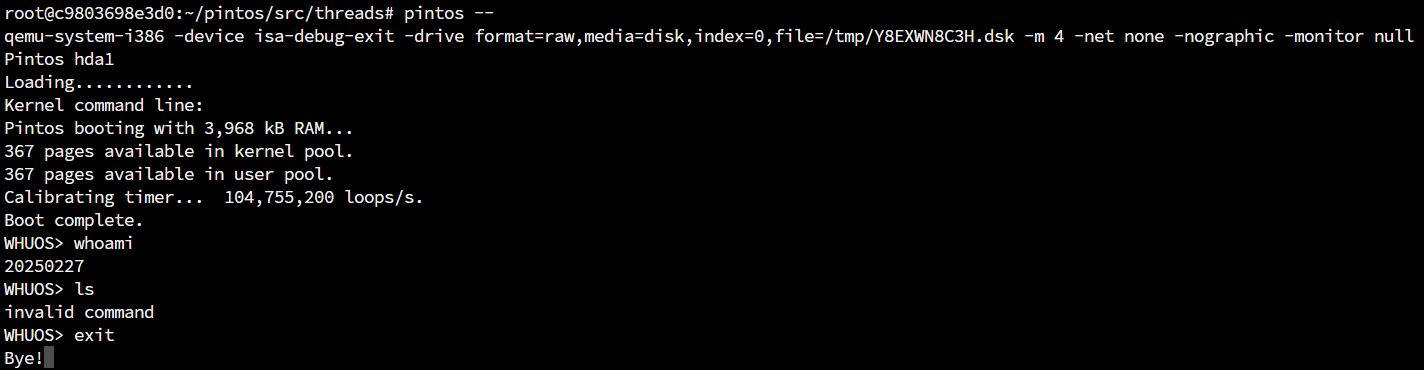
\includegraphics[width=\linewidth]{figure/shell.png}
    \end{figure}
\end{frame}
%---------------------------
\begin{frame}{The End}
    \centering
    \vfill
    \Huge
    \textbf{Thank you!}
    \vfill
    \normalsize
    Any questions?
    \vfill
\end{frame}
\end{document}
